\documentclass[11pt]{article}
\providecommand{\ACLMODE}{review}
\usepackage[\ACLMODE]{acl}
\usepackage{times}
\usepackage{latexsym}
\usepackage[T1]{fontenc}
\usepackage[utf8]{inputenc}
\usepackage{microtype}
\usepackage{inconsolata}
\usepackage{graphicx}
\usepackage{booktabs}
\usepackage{multirow}
\usepackage{amsmath,amssymb}
\usepackage{xcolor}
\usepackage{tikz}
\usetikzlibrary{positioning,arrows.meta,fit}

% Placeholders for content that must come from results/ (never typed by hand).
\newcommand{\todo}[1]{\textcolor{red}{[TODO: #1]}}
\newcommand{\tbc}[1]{\textcolor{blue}{[TEAM TO CONFIRM: #1]}}
% Numbers: macros generated by scripts/summarize.py. \R{Name} uses the test-split value when it exists, else dev.
\newcommand{\EmMZeroDev}{60.3}
\newcommand{\SeedsMZeroDev}{1}
\newcommand{\EmloMZeroDev}{57.3}
\newcommand{\EmhiMZeroDev}{63.4}
\newcommand{\FscoreMZeroDev}{66.9}
\newcommand{\ValidMZeroDev}{100.0}
\newcommand{\HopeffMZeroDev}{61.0}
\newcommand{\HopsMZeroDev}{2.05}
\newcommand{\EmBOneSftDev}{29.1}
\newcommand{\SeedsBOneSftDev}{3}
\newcommand{\EmloBOneSftDev}{27.5}
\newcommand{\EmhiBOneSftDev}{30.8}
\newcommand{\FscoreBOneSftDev}{35.2}
\newcommand{\EmBTwoAGrpoDev}{13.1}
\newcommand{\SeedsBTwoAGrpoDev}{3}
\newcommand{\EmloBTwoAGrpoDev}{11.9}
\newcommand{\EmhiBTwoAGrpoDev}{14.3}
\newcommand{\FscoreBTwoAGrpoDev}{17.6}
\newcommand{\ValidBTwoAGrpoDev}{10.1}
\newcommand{\HopeffBTwoAGrpoDev}{7.2}
\newcommand{\HopsBTwoAGrpoDev}{4.00}
\newcommand{\EmBTwoBGrpoPathDev}{7.1}
\newcommand{\SeedsBTwoBGrpoPathDev}{3}
\newcommand{\EmloBTwoBGrpoPathDev}{6.2}
\newcommand{\EmhiBTwoBGrpoPathDev}{8.1}
\newcommand{\FscoreBTwoBGrpoPathDev}{11.2}
\newcommand{\ValidBTwoBGrpoPathDev}{8.2}
\newcommand{\HopeffBTwoBGrpoPathDev}{3.1}
\newcommand{\HopsBTwoBGrpoPathDev}{4.00}
\newcommand{\EmBThreeSoftDev}{13.1}
\newcommand{\SeedsBThreeSoftDev}{3}
\newcommand{\EmloBThreeSoftDev}{11.9}
\newcommand{\EmhiBThreeSoftDev}{14.3}
\newcommand{\FscoreBThreeSoftDev}{18.1}
\newcommand{\ValidBThreeSoftDev}{7.2}
\newcommand{\HopeffBThreeSoftDev}{9.9}
\newcommand{\HopsBThreeSoftDev}{3.00}
\newcommand{\EmHOneHoppoDev}{10.2}
\newcommand{\SeedsHOneHoppoDev}{3}
\newcommand{\EmloHOneHoppoDev}{9.1}
\newcommand{\EmhiHOneHoppoDev}{11.3}
\newcommand{\FscoreHOneHoppoDev}{14.4}
\newcommand{\ValidHOneHoppoDev}{14.0}
\newcommand{\HopeffHOneHoppoDev}{7.8}
\newcommand{\HopsHOneHoppoDev}{2.69}
\newcommand{\EmAOneTerminalDev}{13.4}
\newcommand{\SeedsAOneTerminalDev}{3}
\newcommand{\EmloAOneTerminalDev}{12.2}
\newcommand{\EmhiAOneTerminalDev}{14.6}
\newcommand{\FscoreAOneTerminalDev}{17.7}
\newcommand{\ValidAOneTerminalDev}{11.7}
\newcommand{\HopeffAOneTerminalDev}{7.2}
\newcommand{\HopsAOneTerminalDev}{4.00}
\newcommand{\EmATwoNoredundDev}{15.5}
\newcommand{\SeedsATwoNoredundDev}{3}
\newcommand{\EmloATwoNoredundDev}{14.2}
\newcommand{\EmhiATwoNoredundDev}{16.8}
\newcommand{\FscoreATwoNoredundDev}{19.9}
\newcommand{\ValidATwoNoredundDev}{17.2}
\newcommand{\HopeffATwoNoredundDev}{10.2}
\newcommand{\HopsATwoNoredundDev}{3.30}
\newcommand{\EmAThreeNoschemaDev}{10.6}
\newcommand{\SeedsAThreeNoschemaDev}{3}
\newcommand{\EmloAThreeNoschemaDev}{9.5}
\newcommand{\EmhiAThreeNoschemaDev}{11.7}
\newcommand{\FscoreAThreeNoschemaDev}{14.9}
\newcommand{\ValidAThreeNoschemaDev}{13.1}
\newcommand{\HopeffAThreeNoschemaDev}{7.0}
\newcommand{\HopsAThreeNoschemaDev}{3.11}
\newcommand{\EmAFourUnrestrictedDev}{10.2}
\newcommand{\SeedsAFourUnrestrictedDev}{3}
\newcommand{\EmloAFourUnrestrictedDev}{9.2}
\newcommand{\EmhiAFourUnrestrictedDev}{11.3}
\newcommand{\FscoreAFourUnrestrictedDev}{14.7}
\newcommand{\ValidAFourUnrestrictedDev}{9.7}
\newcommand{\HopeffAFourUnrestrictedDev}{5.2}
\newcommand{\HopsAFourUnrestrictedDev}{4.00}
\newcommand{\DiffMZeroDev}{-50.1}
\newcommand{\DiffloMZeroDev}{-53.2}
\newcommand{\DiffhiMZeroDev}{-47.1}
\newcommand{\DiffBOneSftDev}{-19.0}
\newcommand{\DiffloBOneSftDev}{-21.9}
\newcommand{\DiffhiBOneSftDev}{-16.1}
\newcommand{\SeeddiffBOneSftDev}{-17.0, -20.2, -19.7}
\newcommand{\SeedagreeBOneSftDev}{yes}
\newcommand{\DiffBTwoAGrpoDev}{-2.9}
\newcommand{\DiffloBTwoAGrpoDev}{-4.1}
\newcommand{\DiffhiBTwoAGrpoDev}{-1.7}
\newcommand{\SeeddiffBTwoAGrpoDev}{-0.3, -6.1, -2.4}
\newcommand{\SeedagreeBTwoAGrpoDev}{yes}
\newcommand{\DiffBTwoBGrpoPathDev}{+3.0}
\newcommand{\DiffloBTwoBGrpoPathDev}{+1.5}
\newcommand{\DiffhiBTwoBGrpoPathDev}{+4.6}
\newcommand{\SeeddiffBTwoBGrpoPathDev}{+4.0, +2.4, +2.7}
\newcommand{\SeedagreeBTwoBGrpoPathDev}{yes}
\newcommand{\DiffBThreeSoftDev}{-2.9}
\newcommand{\DiffloBThreeSoftDev}{-5.0}
\newcommand{\DiffhiBThreeSoftDev}{-0.8}
\newcommand{\SeeddiffBThreeSoftDev}{-2.5, -4.0, -2.2}
\newcommand{\SeedagreeBThreeSoftDev}{yes}
\newcommand{\DiffAOneTerminalDev}{-3.2}
\newcommand{\DiffloAOneTerminalDev}{-4.5}
\newcommand{\DiffhiAOneTerminalDev}{-2.0}
\newcommand{\SeeddiffAOneTerminalDev}{-8.9, -1.3, +0.6}
\newcommand{\SeedagreeAOneTerminalDev}{no}
\newcommand{\DiffATwoNoredundDev}{-5.4}
\newcommand{\DiffloATwoNoredundDev}{-6.8}
\newcommand{\DiffhiATwoNoredundDev}{-3.9}
\newcommand{\SeeddiffATwoNoredundDev}{-6.7, -1.7, -7.7}
\newcommand{\SeedagreeATwoNoredundDev}{yes}
\newcommand{\DiffAThreeNoschemaDev}{-0.4}
\newcommand{\DiffloAThreeNoschemaDev}{-1.5}
\newcommand{\DiffhiAThreeNoschemaDev}{+0.7}
\newcommand{\SeeddiffAThreeNoschemaDev}{+0.5, -1.2, -0.5}
\newcommand{\SeedagreeAThreeNoschemaDev}{no}
\newcommand{\DiffAFourUnrestrictedDev}{-0.1}
\newcommand{\DiffloAFourUnrestrictedDev}{-1.3}
\newcommand{\DiffhiAFourUnrestrictedDev}{+1.2}
\newcommand{\SeeddiffAFourUnrestrictedDev}{-0.5, +0.2, +0.1}
\newcommand{\SeedagreeAFourUnrestrictedDev}{no}
\newcommand{\EmMZeroTest}{57.2}
\newcommand{\SeedsMZeroTest}{1}
\newcommand{\EmloMZeroTest}{55.0}
\newcommand{\EmhiMZeroTest}{59.3}
\newcommand{\FscoreMZeroTest}{64.0}
\newcommand{\ValidMZeroTest}{100.0}
\newcommand{\HopeffMZeroTest}{58.7}
\newcommand{\HopsMZeroTest}{2.06}
\newcommand{\EmBOneSftTest}{27.0}
\newcommand{\SeedsBOneSftTest}{3}
\newcommand{\EmloBOneSftTest}{25.9}
\newcommand{\EmhiBOneSftTest}{28.1}
\newcommand{\FscoreBOneSftTest}{33.3}
\newcommand{\EmBTwoAGrpoTest}{11.5}
\newcommand{\SeedsBTwoAGrpoTest}{3}
\newcommand{\EmloBTwoAGrpoTest}{10.7}
\newcommand{\EmhiBTwoAGrpoTest}{12.3}
\newcommand{\FscoreBTwoAGrpoTest}{15.8}
\newcommand{\ValidBTwoAGrpoTest}{10.5}
\newcommand{\HopeffBTwoAGrpoTest}{6.3}
\newcommand{\HopsBTwoAGrpoTest}{4.00}
\newcommand{\EmBTwoBGrpoPathTest}{6.9}
\newcommand{\SeedsBTwoBGrpoPathTest}{3}
\newcommand{\EmloBTwoBGrpoPathTest}{6.3}
\newcommand{\EmhiBTwoBGrpoPathTest}{7.6}
\newcommand{\FscoreBTwoBGrpoPathTest}{10.8}
\newcommand{\ValidBTwoBGrpoPathTest}{9.0}
\newcommand{\HopeffBTwoBGrpoPathTest}{2.9}
\newcommand{\HopsBTwoBGrpoPathTest}{4.00}
\newcommand{\EmBThreeSoftTest}{11.3}
\newcommand{\SeedsBThreeSoftTest}{3}
\newcommand{\EmloBThreeSoftTest}{10.5}
\newcommand{\EmhiBThreeSoftTest}{12.1}
\newcommand{\FscoreBThreeSoftTest}{15.7}
\newcommand{\ValidBThreeSoftTest}{6.4}
\newcommand{\HopeffBThreeSoftTest}{8.6}
\newcommand{\HopsBThreeSoftTest}{3.00}
\newcommand{\EmHOneHoppoTest}{9.5}
\newcommand{\SeedsHOneHoppoTest}{3}
\newcommand{\EmloHOneHoppoTest}{8.8}
\newcommand{\EmhiHOneHoppoTest}{10.3}
\newcommand{\FscoreHOneHoppoTest}{13.5}
\newcommand{\ValidHOneHoppoTest}{14.0}
\newcommand{\HopeffHOneHoppoTest}{6.9}
\newcommand{\HopsHOneHoppoTest}{2.70}
\newcommand{\EmAOneTerminalTest}{11.9}
\newcommand{\SeedsAOneTerminalTest}{3}
\newcommand{\EmloAOneTerminalTest}{11.0}
\newcommand{\EmhiAOneTerminalTest}{12.7}
\newcommand{\FscoreAOneTerminalTest}{15.8}
\newcommand{\ValidAOneTerminalTest}{12.1}
\newcommand{\HopeffAOneTerminalTest}{6.4}
\newcommand{\HopsAOneTerminalTest}{4.00}
\newcommand{\EmATwoNoredundTest}{14.8}
\newcommand{\SeedsATwoNoredundTest}{3}
\newcommand{\EmloATwoNoredundTest}{13.9}
\newcommand{\EmhiATwoNoredundTest}{15.6}
\newcommand{\FscoreATwoNoredundTest}{19.4}
\newcommand{\ValidATwoNoredundTest}{18.3}
\newcommand{\HopeffATwoNoredundTest}{9.5}
\newcommand{\HopsATwoNoredundTest}{3.30}
\newcommand{\EmAThreeNoschemaTest}{9.1}
\newcommand{\SeedsAThreeNoschemaTest}{3}
\newcommand{\EmloAThreeNoschemaTest}{8.4}
\newcommand{\EmhiAThreeNoschemaTest}{9.8}
\newcommand{\FscoreAThreeNoschemaTest}{13.3}
\newcommand{\ValidAThreeNoschemaTest}{13.4}
\newcommand{\HopeffAThreeNoschemaTest}{5.7}
\newcommand{\HopsAThreeNoschemaTest}{3.10}
\newcommand{\EmAFourUnrestrictedTest}{8.6}
\newcommand{\SeedsAFourUnrestrictedTest}{3}
\newcommand{\EmloAFourUnrestrictedTest}{7.9}
\newcommand{\EmhiAFourUnrestrictedTest}{9.2}
\newcommand{\FscoreAFourUnrestrictedTest}{12.9}
\newcommand{\ValidAFourUnrestrictedTest}{10.0}
\newcommand{\HopeffAFourUnrestrictedTest}{4.2}
\newcommand{\HopsAFourUnrestrictedTest}{4.00}
\newcommand{\DiffMZeroTest}{-47.6}
\newcommand{\DiffloMZeroTest}{-49.7}
\newcommand{\DiffhiMZeroTest}{-45.5}
\newcommand{\DiffBOneSftTest}{-17.5}
\newcommand{\DiffloBOneSftTest}{-19.4}
\newcommand{\DiffhiBOneSftTest}{-15.6}
\newcommand{\SeeddiffBOneSftTest}{-18.2, -18.2, -16.1}
\newcommand{\SeedagreeBOneSftTest}{yes}
\newcommand{\DiffBTwoAGrpoTest}{-2.0}
\newcommand{\DiffloBTwoAGrpoTest}{-2.8}
\newcommand{\DiffhiBTwoAGrpoTest}{-1.2}
\newcommand{\SeeddiffBTwoAGrpoTest}{-1.2, -5.8, +1.0}
\newcommand{\SeedagreeBTwoAGrpoTest}{no}
\newcommand{\DiffBTwoBGrpoPathTest}{+2.6}
\newcommand{\DiffloBTwoBGrpoPathTest}{+1.6}
\newcommand{\DiffhiBTwoBGrpoPathTest}{+3.6}
\newcommand{\SeeddiffBTwoBGrpoPathTest}{+2.2, +1.7, +3.9}
\newcommand{\SeedagreeBTwoBGrpoPathTest}{yes}
\newcommand{\DiffBThreeSoftTest}{-1.8}
\newcommand{\DiffloBThreeSoftTest}{-3.1}
\newcommand{\DiffhiBThreeSoftTest}{-0.5}
\newcommand{\SeeddiffBThreeSoftTest}{-2.8, -3.0, +0.5}
\newcommand{\SeedagreeBThreeSoftTest}{no}
\newcommand{\DiffAOneTerminalTest}{-2.3}
\newcommand{\DiffloAOneTerminalTest}{-3.2}
\newcommand{\DiffhiAOneTerminalTest}{-1.5}
\newcommand{\SeeddiffAOneTerminalTest}{-9.7, -0.1, +2.8}
\newcommand{\SeedagreeAOneTerminalTest}{no}
\newcommand{\DiffATwoNoredundTest}{-5.2}
\newcommand{\DiffloATwoNoredundTest}{-6.2}
\newcommand{\DiffhiATwoNoredundTest}{-4.2}
\newcommand{\SeeddiffATwoNoredundTest}{-9.8, +1.1, -7.0}
\newcommand{\SeedagreeATwoNoredundTest}{no}
\newcommand{\DiffAThreeNoschemaTest}{+0.4}
\newcommand{\DiffloAThreeNoschemaTest}{-0.3}
\newcommand{\DiffhiAThreeNoschemaTest}{+1.1}
\newcommand{\SeeddiffAThreeNoschemaTest}{-2.1, +1.0, +2.3}
\newcommand{\SeedagreeAThreeNoschemaTest}{no}
\newcommand{\DiffAFourUnrestrictedTest}{+1.0}
\newcommand{\DiffloAFourUnrestrictedTest}{+0.1}
\newcommand{\DiffhiAFourUnrestrictedTest}{+1.8}
\newcommand{\SeeddiffAFourUnrestrictedTest}{+0.0, +0.5, +2.3}
\newcommand{\SeedagreeAFourUnrestrictedTest}{yes}
\newcommand{\EmMZeroOodDev}{59.0}
\newcommand{\SeedsMZeroOodDev}{1}
\newcommand{\EmloMZeroOodDev}{54.6}
\newcommand{\EmhiMZeroOodDev}{63.4}
\newcommand{\FscoreMZeroOodDev}{70.2}
\newcommand{\ValidMZeroOodDev}{100.0}
\newcommand{\HopeffMZeroOodDev}{59.6}
\newcommand{\HopsMZeroOodDev}{2.05}
\newcommand{\EmBOneSftOodDev}{29.1}
\newcommand{\SeedsBOneSftOodDev}{3}
\newcommand{\EmloBOneSftOodDev}{26.9}
\newcommand{\EmhiBOneSftOodDev}{31.4}
\newcommand{\FscoreBOneSftOodDev}{38.8}
\newcommand{\EmBTwoAGrpoOodDev}{10.6}
\newcommand{\SeedsBTwoAGrpoOodDev}{3}
\newcommand{\EmloBTwoAGrpoOodDev}{9.1}
\newcommand{\EmhiBTwoAGrpoOodDev}{12.2}
\newcommand{\FscoreBTwoAGrpoOodDev}{16.1}
\newcommand{\ValidBTwoAGrpoOodDev}{10.9}
\newcommand{\HopeffBTwoAGrpoOodDev}{5.5}
\newcommand{\HopsBTwoAGrpoOodDev}{4.00}
\newcommand{\EmBTwoBGrpoPathOodDev}{7.0}
\newcommand{\SeedsBTwoBGrpoPathOodDev}{3}
\newcommand{\EmloBTwoBGrpoPathOodDev}{5.7}
\newcommand{\EmhiBTwoBGrpoPathOodDev}{8.3}
\newcommand{\FscoreBTwoBGrpoPathOodDev}{12.6}
\newcommand{\ValidBTwoBGrpoPathOodDev}{9.5}
\newcommand{\HopeffBTwoBGrpoPathOodDev}{3.2}
\newcommand{\HopsBTwoBGrpoPathOodDev}{4.00}
\newcommand{\EmBThreeSoftOodDev}{11.5}
\newcommand{\SeedsBThreeSoftOodDev}{3}
\newcommand{\EmloBThreeSoftOodDev}{9.9}
\newcommand{\EmhiBThreeSoftOodDev}{13.1}
\newcommand{\FscoreBThreeSoftOodDev}{17.4}
\newcommand{\ValidBThreeSoftOodDev}{8.1}
\newcommand{\HopeffBThreeSoftOodDev}{8.5}
\newcommand{\HopsBThreeSoftOodDev}{3.00}
\newcommand{\EmHOneHoppoOodDev}{9.0}
\newcommand{\SeedsHOneHoppoOodDev}{3}
\newcommand{\EmloHOneHoppoOodDev}{7.6}
\newcommand{\EmhiHOneHoppoOodDev}{10.5}
\newcommand{\FscoreHOneHoppoOodDev}{14.5}
\newcommand{\ValidHOneHoppoOodDev}{15.2}
\newcommand{\HopeffHOneHoppoOodDev}{6.5}
\newcommand{\HopsHOneHoppoOodDev}{2.70}
\newcommand{\EmAOneTerminalOodDev}{10.8}
\newcommand{\SeedsAOneTerminalOodDev}{3}
\newcommand{\EmloAOneTerminalOodDev}{9.3}
\newcommand{\EmhiAOneTerminalOodDev}{12.4}
\newcommand{\FscoreAOneTerminalOodDev}{16.3}
\newcommand{\ValidAOneTerminalOodDev}{12.6}
\newcommand{\HopeffAOneTerminalOodDev}{5.9}
\newcommand{\HopsAOneTerminalOodDev}{4.00}
\newcommand{\EmATwoNoredundOodDev}{13.9}
\newcommand{\SeedsATwoNoredundOodDev}{3}
\newcommand{\EmloATwoNoredundOodDev}{12.1}
\newcommand{\EmhiATwoNoredundOodDev}{15.6}
\newcommand{\FscoreATwoNoredundOodDev}{19.7}
\newcommand{\ValidATwoNoredundOodDev}{18.1}
\newcommand{\HopeffATwoNoredundOodDev}{8.9}
\newcommand{\HopsATwoNoredundOodDev}{3.31}
\newcommand{\EmAThreeNoschemaOodDev}{8.4}
\newcommand{\SeedsAThreeNoschemaOodDev}{3}
\newcommand{\EmloAThreeNoschemaOodDev}{7.0}
\newcommand{\EmhiAThreeNoschemaOodDev}{9.8}
\newcommand{\FscoreAThreeNoschemaOodDev}{14.0}
\newcommand{\ValidAThreeNoschemaOodDev}{13.9}
\newcommand{\HopeffAThreeNoschemaOodDev}{5.4}
\newcommand{\HopsAThreeNoschemaOodDev}{3.15}
\newcommand{\EmAFourUnrestrictedOodDev}{8.6}
\newcommand{\SeedsAFourUnrestrictedOodDev}{3}
\newcommand{\EmloAFourUnrestrictedOodDev}{7.3}
\newcommand{\EmhiAFourUnrestrictedOodDev}{10.0}
\newcommand{\FscoreAFourUnrestrictedOodDev}{14.5}
\newcommand{\ValidAFourUnrestrictedOodDev}{10.3}
\newcommand{\HopeffAFourUnrestrictedOodDev}{4.2}
\newcommand{\HopsAFourUnrestrictedOodDev}{4.00}
\newcommand{\DiffMZeroOodDev}{-50.0}
\newcommand{\DiffloMZeroOodDev}{-54.2}
\newcommand{\DiffhiMZeroOodDev}{-45.8}
\newcommand{\DiffBOneSftOodDev}{-20.1}
\newcommand{\DiffloBOneSftOodDev}{-23.9}
\newcommand{\DiffhiBOneSftOodDev}{-16.3}
\newcommand{\SeeddiffBOneSftOodDev}{-19.8, -20.6, -20.0}
\newcommand{\SeedagreeBOneSftOodDev}{yes}
\newcommand{\DiffBTwoAGrpoOodDev}{-1.6}
\newcommand{\DiffloBTwoAGrpoOodDev}{-3.1}
\newcommand{\DiffhiBTwoAGrpoOodDev}{-0.1}
\newcommand{\SeeddiffBTwoAGrpoOodDev}{-0.6, -4.8, +0.6}
\newcommand{\SeedagreeBTwoAGrpoOodDev}{no}
\newcommand{\DiffBTwoBGrpoPathOodDev}{+2.0}
\newcommand{\DiffloBTwoBGrpoPathOodDev}{-0.0}
\newcommand{\DiffhiBTwoBGrpoPathOodDev}{+4.1}
\newcommand{\SeeddiffBTwoBGrpoPathOodDev}{+1.8, +1.8, +2.4}
\newcommand{\SeedagreeBTwoBGrpoPathOodDev}{yes}
\newcommand{\DiffBThreeSoftOodDev}{-2.5}
\newcommand{\DiffloBThreeSoftOodDev}{-5.1}
\newcommand{\DiffhiBThreeSoftOodDev}{+0.0}
\newcommand{\SeeddiffBThreeSoftOodDev}{-3.4, -4.0, -0.2}
\newcommand{\SeedagreeBThreeSoftOodDev}{yes}
\newcommand{\DiffAOneTerminalOodDev}{-1.8}
\newcommand{\DiffloAOneTerminalOodDev}{-3.6}
\newcommand{\DiffhiAOneTerminalOodDev}{+0.0}
\newcommand{\SeeddiffAOneTerminalOodDev}{-6.6, -1.4, +2.6}
\newcommand{\SeedagreeAOneTerminalOodDev}{no}
\newcommand{\DiffATwoNoredundOodDev}{-4.9}
\newcommand{\DiffloATwoNoredundOodDev}{-6.8}
\newcommand{\DiffhiATwoNoredundOodDev}{-2.9}
\newcommand{\SeeddiffATwoNoredundOodDev}{-7.6, -1.4, -5.6}
\newcommand{\SeedagreeATwoNoredundOodDev}{yes}
\newcommand{\DiffAThreeNoschemaOodDev}{+0.6}
\newcommand{\DiffloAThreeNoschemaOodDev}{-0.7}
\newcommand{\DiffhiAThreeNoschemaOodDev}{+1.9}
\newcommand{\SeeddiffAThreeNoschemaOodDev}{+1.2, -0.2, +0.8}
\newcommand{\SeedagreeAThreeNoschemaOodDev}{no}
\newcommand{\DiffAFourUnrestrictedOodDev}{+0.4}
\newcommand{\DiffloAFourUnrestrictedOodDev}{-1.3}
\newcommand{\DiffhiAFourUnrestrictedOodDev}{+2.1}
\newcommand{\SeeddiffAFourUnrestrictedOodDev}{-0.4, +0.6, +1.0}
\newcommand{\SeedagreeAFourUnrestrictedOodDev}{no}
\newcommand{\EmMZeroOodTest}{53.1}
\newcommand{\SeedsMZeroOodTest}{1}
\newcommand{\EmloMZeroOodTest}{48.9}
\newcommand{\EmhiMZeroOodTest}{57.1}
\newcommand{\FscoreMZeroOodTest}{61.8}
\newcommand{\ValidMZeroOodTest}{100.0}
\newcommand{\HopeffMZeroOodTest}{55.2}
\newcommand{\HopsMZeroOodTest}{2.05}
\newcommand{\EmBOneSftOodTest}{23.1}
\newcommand{\SeedsBOneSftOodTest}{3}
\newcommand{\EmloBOneSftOodTest}{21.1}
\newcommand{\EmhiBOneSftOodTest}{25.1}
\newcommand{\FscoreBOneSftOodTest}{29.8}
\newcommand{\EmBTwoAGrpoOodTest}{9.8}
\newcommand{\SeedsBTwoAGrpoOodTest}{3}
\newcommand{\EmloBTwoAGrpoOodTest}{8.4}
\newcommand{\EmhiBTwoAGrpoOodTest}{11.2}
\newcommand{\FscoreBTwoAGrpoOodTest}{14.1}
\newcommand{\ValidBTwoAGrpoOodTest}{10.9}
\newcommand{\HopeffBTwoAGrpoOodTest}{5.4}
\newcommand{\HopsBTwoAGrpoOodTest}{4.00}
\newcommand{\EmBTwoBGrpoPathOodTest}{6.4}
\newcommand{\SeedsBTwoBGrpoPathOodTest}{3}
\newcommand{\EmloBTwoBGrpoPathOodTest}{5.3}
\newcommand{\EmhiBTwoBGrpoPathOodTest}{7.6}
\newcommand{\FscoreBTwoBGrpoPathOodTest}{11.6}
\newcommand{\ValidBTwoBGrpoPathOodTest}{9.2}
\newcommand{\HopeffBTwoBGrpoPathOodTest}{2.8}
\newcommand{\HopsBTwoBGrpoPathOodTest}{4.00}
\newcommand{\EmBThreeSoftOodTest}{9.6}
\newcommand{\SeedsBThreeSoftOodTest}{3}
\newcommand{\EmloBThreeSoftOodTest}{8.3}
\newcommand{\EmhiBThreeSoftOodTest}{11.0}
\newcommand{\FscoreBThreeSoftOodTest}{14.3}
\newcommand{\ValidBThreeSoftOodTest}{6.9}
\newcommand{\HopeffBThreeSoftOodTest}{7.8}
\newcommand{\HopsBThreeSoftOodTest}{3.00}
\newcommand{\EmHOneHoppoOodTest}{9.0}
\newcommand{\SeedsHOneHoppoOodTest}{3}
\newcommand{\EmloHOneHoppoOodTest}{7.6}
\newcommand{\EmhiHOneHoppoOodTest}{10.3}
\newcommand{\FscoreHOneHoppoOodTest}{13.5}
\newcommand{\ValidHOneHoppoOodTest}{15.8}
\newcommand{\HopeffHOneHoppoOodTest}{7.4}
\newcommand{\HopsHOneHoppoOodTest}{2.70}
\newcommand{\EmAOneTerminalOodTest}{9.9}
\newcommand{\SeedsAOneTerminalOodTest}{3}
\newcommand{\EmloAOneTerminalOodTest}{8.5}
\newcommand{\EmhiAOneTerminalOodTest}{11.4}
\newcommand{\FscoreAOneTerminalOodTest}{14.6}
\newcommand{\ValidAOneTerminalOodTest}{12.6}
\newcommand{\HopeffAOneTerminalOodTest}{5.7}
\newcommand{\HopsAOneTerminalOodTest}{4.00}
\newcommand{\EmATwoNoredundOodTest}{11.8}
\newcommand{\SeedsATwoNoredundOodTest}{3}
\newcommand{\EmloATwoNoredundOodTest}{10.3}
\newcommand{\EmhiATwoNoredundOodTest}{13.3}
\newcommand{\FscoreATwoNoredundOodTest}{17.1}
\newcommand{\ValidATwoNoredundOodTest}{18.0}
\newcommand{\HopeffATwoNoredundOodTest}{8.0}
\newcommand{\HopsATwoNoredundOodTest}{3.32}
\newcommand{\EmAThreeNoschemaOodTest}{7.4}
\newcommand{\SeedsAThreeNoschemaOodTest}{3}
\newcommand{\EmloAThreeNoschemaOodTest}{6.2}
\newcommand{\EmhiAThreeNoschemaOodTest}{8.7}
\newcommand{\FscoreAThreeNoschemaOodTest}{11.9}
\newcommand{\ValidAThreeNoschemaOodTest}{14.0}
\newcommand{\HopeffAThreeNoschemaOodTest}{5.1}
\newcommand{\HopsAThreeNoschemaOodTest}{3.18}
\newcommand{\EmAFourUnrestrictedOodTest}{8.4}
\newcommand{\SeedsAFourUnrestrictedOodTest}{3}
\newcommand{\EmloAFourUnrestrictedOodTest}{7.1}
\newcommand{\EmhiAFourUnrestrictedOodTest}{9.8}
\newcommand{\FscoreAFourUnrestrictedOodTest}{13.2}
\newcommand{\ValidAFourUnrestrictedOodTest}{10.9}
\newcommand{\HopeffAFourUnrestrictedOodTest}{4.5}
\newcommand{\HopsAFourUnrestrictedOodTest}{4.00}
\newcommand{\DiffMZeroOodTest}{-44.1}
\newcommand{\DiffloMZeroOodTest}{-48.0}
\newcommand{\DiffhiMZeroOodTest}{-40.1}
\newcommand{\DiffBOneSftOodTest}{-14.1}
\newcommand{\DiffloBOneSftOodTest}{-17.5}
\newcommand{\DiffhiBOneSftOodTest}{-10.7}
\newcommand{\SeeddiffBOneSftOodTest}{-12.7, -14.1, -15.6}
\newcommand{\SeedagreeBOneSftOodTest}{yes}
\newcommand{\DiffBTwoAGrpoOodTest}{-0.8}
\newcommand{\DiffloBTwoAGrpoOodTest}{-2.2}
\newcommand{\DiffhiBTwoAGrpoOodTest}{+0.6}
\newcommand{\SeeddiffBTwoAGrpoOodTest}{+2.3, -3.2, -1.6}
\newcommand{\SeedagreeBTwoAGrpoOodTest}{no}
\newcommand{\DiffBTwoBGrpoPathOodTest}{+2.5}
\newcommand{\DiffloBTwoBGrpoPathOodTest}{+0.6}
\newcommand{\DiffhiBTwoBGrpoPathOodTest}{+4.5}
\newcommand{\SeeddiffBTwoBGrpoPathOodTest}{+4.4, +3.2, +0.0}
\newcommand{\SeedagreeBTwoBGrpoPathOodTest}{no}
\newcommand{\DiffBThreeSoftOodTest}{-0.6}
\newcommand{\DiffloBThreeSoftOodTest}{-3.2}
\newcommand{\DiffhiBThreeSoftOodTest}{+1.9}
\newcommand{\SeeddiffBThreeSoftOodTest}{+0.4, +0.4, -2.6}
\newcommand{\SeedagreeBThreeSoftOodTest}{no}
\newcommand{\DiffAOneTerminalOodTest}{-0.9}
\newcommand{\DiffloAOneTerminalOodTest}{-2.3}
\newcommand{\DiffhiAOneTerminalOodTest}{+0.4}
\newcommand{\SeeddiffAOneTerminalOodTest}{-4.4, +1.1, +0.5}
\newcommand{\SeedagreeAOneTerminalOodTest}{no}
\newcommand{\DiffATwoNoredundOodTest}{-2.8}
\newcommand{\DiffloATwoNoredundOodTest}{-4.5}
\newcommand{\DiffhiATwoNoredundOodTest}{-1.2}
\newcommand{\SeeddiffATwoNoredundOodTest}{-4.2, +1.9, -6.2}
\newcommand{\SeedagreeATwoNoredundOodTest}{no}
\newcommand{\DiffAThreeNoschemaOodTest}{+1.6}
\newcommand{\DiffloAThreeNoschemaOodTest}{+0.5}
\newcommand{\DiffhiAThreeNoschemaOodTest}{+2.7}
\newcommand{\SeeddiffAThreeNoschemaOodTest}{+3.7, +2.1, -1.1}
\newcommand{\SeedagreeAThreeNoschemaOodTest}{no}
\newcommand{\DiffAFourUnrestrictedOodTest}{+0.5}
\newcommand{\DiffloAFourUnrestrictedOodTest}{-0.9}
\newcommand{\DiffhiAFourUnrestrictedOodTest}{+2.1}
\newcommand{\SeeddiffAFourUnrestrictedOodTest}{+1.1, +1.6, -1.1}
\newcommand{\SeedagreeAFourUnrestrictedOodTest}{no}
\newcommand{\GapMZeroOodDev}{1.3}
\newcommand{\GaprelMZeroOodDev}{2.2}
\newcommand{\OodemMZeroOodDev}{59.0}
\newcommand{\GapMZeroOodTest}{4.1}
\newcommand{\GaprelMZeroOodTest}{7.2}
\newcommand{\OodemMZeroOodTest}{53.1}
\newcommand{\GapBOneSftOodDev}{0.0}
\newcommand{\GaprelBOneSftOodDev}{0.0}
\newcommand{\OodemBOneSftOodDev}{29.1}
\newcommand{\GapBOneSftOodTest}{3.9}
\newcommand{\GaprelBOneSftOodTest}{14.6}
\newcommand{\OodemBOneSftOodTest}{23.1}
\newcommand{\GapBTwoAGrpoOodDev}{2.5}
\newcommand{\GaprelBTwoAGrpoOodDev}{19.1}
\newcommand{\OodemBTwoAGrpoOodDev}{10.6}
\newcommand{\GapBTwoAGrpoOodTest}{1.7}
\newcommand{\GaprelBTwoAGrpoOodTest}{14.9}
\newcommand{\OodemBTwoAGrpoOodTest}{9.8}
\newcommand{\GapBTwoBGrpoPathOodDev}{0.1}
\newcommand{\GaprelBTwoBGrpoPathOodDev}{1.9}
\newcommand{\OodemBTwoBGrpoPathOodDev}{7.0}
\newcommand{\GapBTwoBGrpoPathOodTest}{0.5}
\newcommand{\GaprelBTwoBGrpoPathOodTest}{7.2}
\newcommand{\OodemBTwoBGrpoPathOodTest}{6.4}
\newcommand{\GapBThreeSoftOodDev}{1.5}
\newcommand{\GaprelBThreeSoftOodDev}{11.7}
\newcommand{\OodemBThreeSoftOodDev}{11.5}
\newcommand{\GapBThreeSoftOodTest}{1.7}
\newcommand{\GaprelBThreeSoftOodTest}{14.9}
\newcommand{\OodemBThreeSoftOodTest}{9.6}
\newcommand{\GapHOneHoppoOodDev}{1.2}
\newcommand{\GaprelHOneHoppoOodDev}{11.5}
\newcommand{\OodemHOneHoppoOodDev}{9.0}
\newcommand{\GapHOneHoppoOodTest}{0.6}
\newcommand{\GaprelHOneHoppoOodTest}{5.8}
\newcommand{\OodemHOneHoppoOodTest}{9.0}
\newcommand{\GapAOneTerminalOodDev}{2.6}
\newcommand{\GaprelAOneTerminalOodDev}{19.2}
\newcommand{\OodemAOneTerminalOodDev}{10.8}
\newcommand{\GapAOneTerminalOodTest}{1.9}
\newcommand{\GaprelAOneTerminalOodTest}{16.5}
\newcommand{\OodemAOneTerminalOodTest}{9.9}
\newcommand{\GapATwoNoredundOodDev}{1.7}
\newcommand{\GaprelATwoNoredundOodDev}{10.7}
\newcommand{\OodemATwoNoredundOodDev}{13.9}
\newcommand{\GapATwoNoredundOodTest}{3.0}
\newcommand{\GaprelATwoNoredundOodTest}{20.2}
\newcommand{\OodemATwoNoredundOodTest}{11.8}
\newcommand{\GapAThreeNoschemaOodDev}{2.2}
\newcommand{\GaprelAThreeNoschemaOodDev}{20.5}
\newcommand{\OodemAThreeNoschemaOodDev}{8.4}
\newcommand{\GapAThreeNoschemaOodTest}{1.7}
\newcommand{\GaprelAThreeNoschemaOodTest}{19.0}
\newcommand{\OodemAThreeNoschemaOodTest}{7.4}
\newcommand{\GapAFourUnrestrictedOodDev}{1.6}
\newcommand{\GaprelAFourUnrestrictedOodDev}{16.0}
\newcommand{\OodemAFourUnrestrictedOodDev}{8.6}
\newcommand{\GapAFourUnrestrictedOodTest}{0.1}
\newcommand{\GaprelAFourUnrestrictedOodTest}{1.4}
\newcommand{\OodemAFourUnrestrictedOodTest}{8.4}
\newcommand{\GoldCovTrain}{99.1}
\newcommand{\PathLenTrain}{2.05}
\newcommand{\LastEntAnsTrain}{97.8}
\newcommand{\PassageAnsTrain}{56.1}
\newcommand{\RecallKDev}{83.4}
\newcommand{\SanityEm}{95.5}
\newcommand{\SanityValid}{78.1}

\newcommand{\R}[1]{\ifcsname #1Test\endcsname\csname #1Test\endcsname\else\ifcsname #1Dev\endcsname\csname #1Dev\endcsname\else\textbf{??}\fi\fi}
\newcommand{\splitname}{\ifcsname EmHOneHoppoTest\endcsname test\else development\fi}
\newcommand{\CI}[1]{[\R{Emlo#1}, \R{Emhi#1}]}
\newcommand{\D}[1]{\R{Diff#1} [\R{Difflo#1}, \R{Diffhi#1}]}
% Include a figure only if the plotting script has produced it.
\newcommand{\figfile}[2]{\IfFileExists{../results/figures/#1.pdf}{\includegraphics[#2]{../results/figures/#1.pdf}}{\todo{figure \detokenize{#1} not yet generated}}}

\newcommand{\codelink}{\textcolor{blue}{[CODE LINK]}}  % placeholder: repository URL, to be provided
\newcommand{\method}{TableHop-PPO}
\newcommand{\hop}{Hop-PPO}

\title{When Does Hop-Level Credit Help? PPO-Based Entity Selection\\for Multi-Hop Table Question Answering}

\author{Dhruv Goyal \and Shaurya Goyal \\
  \tbc{affiliation, email} \\}

\begin{document}
\maketitle

\begin{abstract}
Multi-hop question answering over tables and linked text requires a chain of intermediate lookups, yet reinforcement learning for table reasoning typically rewards only the final answer, so credit for a correct early lookup is diluted over the whole trace.
We cast each hop as a discrete entity-selection action (a table cell, a linked passage, or STOP) in a partially observable decision process and train the selection policy with proximal policy optimization (PPO) under a hybrid reward that combines a hop-level term with a terminal answer reward.
A frozen answer head reads the selected evidence and produces the answer.
We compare this agent, under matched rollout and tuning budgets and with a shared encoder, candidate set and answer head, against supervised fine-tuning, trace-level group-relative RL with and without gold-path supervision, a soft attention-based selector, and four reward and action-space ablations on HybridQA, including a split with held-out table clusters.
On the \splitname\ split, supervised fine-tuning that reads the whole table remains the strongest method (\R{EmBOneSft} EM versus \R{EmHOneHoppo} for \hop; oracle evidence gives \R{EmMZero}).
Among path-based learners, \hop\ produces the most valid paths (\R{ValidHOneHoppo}\% strict validity) and beats trace-level RL with the same path supervision (\D{BTwoBGrpoPath} EM points), but its EM is not reliably different from answer-only trace-level RL (\D{BTwoAGrpo}).
The dense hop reward does not improve accuracy: the same policy trained with the terminal reward only reaches \R{EmAOneTerminal} EM, because hop rewards teach the policy to stop after about two hops and the frozen reader then sees less evidence.
All experiments run on a single laptop (Apple M4, no discrete GPU) with small frozen backbones, so our conclusions concern this regime and not large language models.
\end{abstract}

\section{Introduction}
\label{sec:intro}

Many questions over semi-structured data cannot be answered from a single cell.
In HybridQA \citep{chen2020hybridqa}, for example, a question may require locating a row through one cell, following a hyperlink from that cell to a passage, and reading the answer there.
Methods that treat table question answering as sequence generation or cell classification \citep{herzig2020tapas,liu2022tapex,zhang2024tablellama} do not expose these intermediate decisions, and recent reinforcement learning (RL) recipes for tables assign one verifiable reward to an entire response \citep{yang2025tabler1,lei2025reasoningtable}.
When a trace has several lookups and only the final answer is scored, a correct first lookup followed by a wrong second lookup receives the same signal as two wrong lookups.
This credit-assignment problem is well studied in RL \citep{ng1999shaping,arjona2019rudder} and in knowledge-graph path reasoning, where shaped rewards help an agent that walks entity by entity \citep{xiong2017deeppath,das2018minerva,lin2018multihop}.
It has received less attention for tables.

We ask a deliberately empirical question: \emph{when does hop-level credit help multi-hop table reasoning?}
We formulate each hop as a discrete choice among a small set of candidate entities (cells, linked passages, STOP), train the choice policy with PPO \citep{schulman2017ppo} using a hybrid reward with hop-level and terminal parts, and let a frozen answer head produce the answer from the selected evidence.
Because a hop-level reward uses gold-path labels, a fair comparison must separate the effect of credit assignment from the effect of extra supervision.
We therefore include a trace-level RL baseline that also receives path supervision, but only at the end of the trace, in addition to a standard answer-only trace-level baseline.

Our contributions are as follows.
\begin{itemize}\setlength\itemsep{0pt}
  \item A controlled environment for multi-hop table QA in which the action space, encoder, candidate generator and answer head are identical for all path-based methods, so that only the learning signal differs (Sections~\ref{sec:formulation}--\ref{sec:method}).
  \item A comparison under matched rollout budget (48{,}000 trajectories) and matched tuning budget against SFT, trace-level GRPO-style RL with and without gold-path supervision, and a soft selector, plus reward ablations and an out-of-domain split built from held-out table clusters (Section~\ref{sec:setup}).
  \item An analysis of accuracy, path validity and hop efficiency with bootstrap confidence intervals, together with the negative results and limitations of a small-scale, noisy-label setting (Sections~\ref{sec:results}--\ref{sec:limitations}).
\end{itemize}
In short, hop-level credit made the policy's paths shorter and more often correct, and it beat trace-level RL that receives the same path signal only at the end; it did not make answers more accurate than an answer-only reward, and no path-based method approached full-table SFT at our scale (Section~\ref{sec:results}; hypothesis status in Table~\ref{tab:claims}).
Our code and data processing scripts are available at \codelink.

\section{Related Work}
\label{sec:related}

\paragraph{Table reasoning.}
Early neural table QA selects cells and an aggregation operator from weak supervision \citep{herzig2020tapas} or pretrains a sequence model to imitate a SQL executor \citep{liu2022tapex}.
Instruction-tuned generalist models cover many table tasks \citep{zhang2024tablellama}.
Prompting methods decompose evidence and questions \citep{ye2023dater}, call symbolic programs that may themselves invoke a language model \citep{cheng2023binder}, or evolve the table through a chain of operations \citep{wang2024chainoftable}.
These approaches either give no learned signal for intermediate steps or operate on prompted language models; ours learns a small selection policy over explicit candidates.

\paragraph{RL for tables and text-based credit assignment.}
Table-R1 \citep{yang2025tabler1} applies RL with verifiable rewards to table tasks and obtains one reward per full response, and Reasoning-Table \citep{lei2025reasoningtable} studies outcome-based RL for table reasoning and text-to-SQL.
Our trace-level baselines B2a and B2b mirror this outcome-reward setting inside our controlled environment; we do not reproduce these systems, which use much larger language models, and do not compare against their published numbers.
In mathematical reasoning, process-level supervision has been compared with outcome-level supervision \citep{uesato2022process,lightman2023verify}; our hop reward plays the role of a process signal, but it is computed from heuristic gold paths rather than human step labels.

\paragraph{RL for multi-hop reasoning on graphs.}
DeepPath \citep{xiong2017deeppath} and MINERVA \citep{das2018minerva} frame knowledge-graph reasoning as walks driven by a learned policy, and reward shaping addresses sparse and misleading terminal signals in this setting \citep{lin2018multihop}.
Later work continues this line for temporal and sparse knowledge graphs \citep{bai2024matpath,liu2025maskgr}.
We port the entity-by-entity view to tables and linked text; we do not implement the multi-agent variants of these later works and cite them as related background only.

\paragraph{Reward shaping and policy optimization.}
Potential-based shaping preserves optimal policies \citep{ng1999shaping}, whereas our hybrid reward is not potential-based and can change the optimum; we test this through ablations rather than assume it helps.
RUDDER decomposes delayed returns \citep{arjona2019rudder}.
We optimize with PPO and generalized advantage estimation \citep{schulman2017ppo,schulman2016gae}, and our trace-level baselines use Group Relative Policy Optimization (GRPO), the PPO variant introduced by \citet{shao2024deepseekmath}, which replaces the value function with group-normalized returns.

\section{Problem Formulation}
\label{sec:formulation}

An example consists of a question $q$, a table $T$ with $R$ rows and $C$ columns whose cells may carry hyperlinks to passages, and the set of linked passages $P$.
Let $\mathcal{E}$ denote the entity set, consisting of the cells of $T$ and the passages in $P$.
The answer is a string $a^\ast$.
Gold answers are available only for training and evaluation; the agent observes neither $a^\ast$ nor any gold path at test time.

We model answering as a finite-horizon, partially observable decision process $(\mathcal{S},\mathcal{A},\mathcal{O},\mathcal{T},r,H)$.
The latent state $s_t$ contains the full example and the trace $\tau_t=(e_1,\dots,e_t)$ of entities selected so far.
The observation $o_t$ contains $q$, an embedding of each selected entity, and the current candidate set $\mathcal{C}_t\subseteq\mathcal{E}\cup\{\textsc{stop}\}$ with relation types and features.
The action $a_t\in\mathcal{C}_t$ selects the next entity or STOP.
Transitions are deterministic: selecting an entity appends it to the trace and, unless $t+1=H$, recomputes the candidate set from the new entity (Section~\ref{sec:method}); the episode ends on STOP, on reaching $H$ hops (forced stop), or on an illegal action.
At termination a frozen answer head $f$ maps $(q,\tau)$ to a predicted answer $\hat a=f(q,\tau)$.
The reward is the sum of per-hop terms $r_t$ and a terminal term $r_T$ (Section~\ref{sec:method}).
We optimize $\pi_\theta(a_t\mid o_t)$ to maximize expected return.
Table~\ref{tab:notation} lists the notation.

\begin{table}[t]
\centering\small
\begin{tabular}{@{}ll@{}}
\toprule
Symbol & Meaning \\
\midrule
$q$, $T$, $P$ & question, table, linked passages \\
$\mathcal{E}$ & entities: cells and passages \\
$H$ & maximum number of hops ($H=4$) \\
$\mathcal{C}_t$ & legal candidates at hop $t$ (incl.\ STOP) \\
$\tau_t=(e_1..e_t)$ & selected entities (trace) \\
$g=(g_1..g_m)$ & heuristic gold path \\
$f$ & frozen answer head, $\hat a=f(q,\tau)$ \\
$\pi_\theta$, $V_\phi$ & policy and value function \\
$r_t$, $r_T$ & hop reward, terminal reward \\
$w_\bullet$ & reward weights (Table~\ref{tab:reward-weights}) \\
\bottomrule
\end{tabular}
\caption{Notation.}
\label{tab:notation}
\end{table}

\section{Method}
\label{sec:method}

Figure~\ref{fig:pipeline} summarizes the pipeline.

\begin{figure*}[t]
\centering
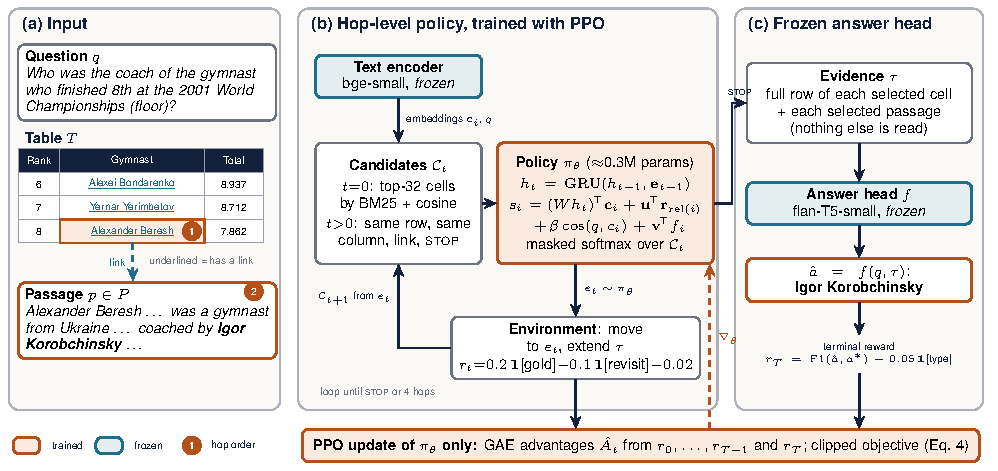
\includegraphics[width=\textwidth]{figures/architecture.pdf}
\caption{\hop\ architecture, shown on a HybridQA dev question. (a) Input: question, table and linked passages; numbers mark the hops taken. (b) The policy $\pi_\theta$, the only trained component, picks one candidate (cell, linked passage or \textsc{stop}) per hop; the environment returns the hop reward $r_t$ and the next candidate set. (c) On \textsc{stop}, the frozen answer head reads only the selected evidence $\tau$; its answer gives the terminal reward $r_T$. PPO updates $\pi_\theta$ from $r_0,\dots,r_T$. All path-based methods share every component except the learning signal.}
\label{fig:pipeline}
\end{figure*}

\subsection{Environment and candidates}
The encoder is the frozen sentence model \texttt{BAAI/bge-small-en-v1.5}; every entity and the question are embedded once and cached.
A cell is rendered as ``table title | column header | row anchor | cell text'', where the row anchor is the first non-numeric cell of the row; a passage is rendered as its title and first 400 characters.
At hop 0 the candidates are the top $K=32$ cells of the table by $0.5\cdot\mathrm{bm25}+0.5\cdot\cos(q,c)$ (BM25 min--max normalized within the table); STOP is illegal at $t=0$.
At later hops the candidates are all cells in the row of the current entity, the 8 cells of its column most similar to $q$, the passage linked from the current cell if there is one, and STOP.
A passage entity inherits the row and column of its source cell.
Re-selecting an entity is legal but flagged as redundant.
The episode ends on STOP, after $H=4$ selected entities (forced stop), or immediately on an illegal action.
The unrestricted variant A4 replaces the row/column neighbourhood at $t>0$ with the top-$K$ cells of the whole table by cosine similarity plus the linked passage and STOP.

\subsection{Policy}
The policy ($\approx$0.3M parameters, trained on CPU) keeps a GRU state $s_t$ over the embeddings of the selected entities, initialized as $s_0=\tanh(W_q q)$.
The logit of candidate $i$ with embedding $c_i$, relation type $\rho_i\in\{\text{start, same-row, same-column, link, stop}\}$ and feature vector $\phi_i$ is
\begin{equation}
\begin{split}\ell_i={}&(Ws_t)^\top c_i+u(s_t)^\top \mathrm{emb}(\rho_i)+\beta\cos(q,c_i)\\&+v^\top\phi_i+\tanh(F\phi_i)^\top g(s_t),\end{split}
\end{equation}
with illegal candidates masked before the softmax; a value head $V_\phi(s_t)$ is an MLP on $s_t$.
The features $\phi_i$ (Appendix~\ref{app:changes}) are the cosine similarity, the normalized BM25 score, the question-token overlap with the entity text and the question-token overlap with the column header (the last two lexical; passages have no BM25 score or header).
They are given identically to H1, A1--A4, B2a, B2b and, as a scorer input, to B3.

\subsection{Hybrid reward}
Let $g$ be the gold path.
For a legal hop that selects entity $e_t$:
\begin{equation}
\begin{split}r_t={}&w_{\text{hop}}\,\mathbb{1}[e_t\in g,\ \text{ordered, new}]\\&-w_{\text{red}}\,\mathbb{1}[e_t\text{ revisited}]-w_{\text{step}}.\end{split}
\end{equation}
\emph{Order-consistent} means the gold index of $e_t$ is not smaller than the largest gold index matched so far; a revisit never re-earns $w_{\text{hop}}$ (an exploit found and fixed during review).
STOP itself earns nothing.
At termination, with $\hat a=f(q,\tau)$,
\begin{equation}
\begin{split}r_T={}&w_{\text{ans}}\,\mathrm{F1}(\hat a,a^\ast)\\&-w_{\text{schema}}\,\mathbb{1}[\text{last cell schema-inconsistent}].\end{split}
\end{equation}
The schema rule uses fixed question cues: a cue such as ``how many'' or ``percent'' requires the last selected cell to have numeric type, and a date cue such as ``what year'' requires a date or number; questions without a cue impose no constraint, and passages are never penalized.
For questions without a gold path ($1.7\%$ of all questions, Appendix~\ref{app:data}) the hop term is zero.
Default weights are $w_{\text{ans}}=1$, $w_{\text{hop}}=0.2$, $w_{\text{red}}=0.1$, $w_{\text{schema}}=0.05$, $w_{\text{step}}=0.02$ and were fixed before training (Table~\ref{tab:reward-weights}).

\subsection{PPO training}
We use a custom clipped-objective PPO with GAE ($\gamma=1$, $\lambda=0.95$), clip $0.2$, value coefficient $0.5$, entropy coefficient $0.01$ decayed linearly to zero, 4 epochs of minibatches of 256 steps per update, per-batch advantage normalization, gradient-norm clipping at $0.5$, Adam with learning rate $3\times10^{-4}$, and 64 single-trajectory episodes per update.
The terminal reward is added to the last step of each trajectory.
The training budget is 48{,}000 trajectories (750 updates).
Variants A1--A4 change only the reward switches or the action space: A1 uses the terminal answer reward only, A2 removes the redundancy penalty, A3 removes the schema term and A4 uses the unrestricted action space.

\subsection{Frozen answer head and row evidence}
The answer head is \texttt{google/flan-t5-small}, fine-tuned once on gold-path evidence (3 epochs, learning rate $3\times10^{-4}$) with distractor entities inserted into 30\% of training examples so that it tolerates imperfect selections, and then frozen for all path-based methods.
Its input is ``question: $q$ evidence: $x_1\,\|\,x_2\dots$'' truncated to 512 tokens, where the evidence $x_j$ is the rendering of the selected entities.
In the final configuration (Appendix~\ref{app:changes}) every selected cell is rendered as its whole row, once per row in first-visit order, and every selected passage as its title and text; passages enter the input only if the policy selects them.
Hence the answer head can read the answer from the row of a selected cell, and a policy that selects a good first cell can already earn answer reward, whereas passage answers require the link hop.

\section{Experimental Setup}
\label{sec:setup}

\paragraph{Data and splits.}
We use HybridQA \citep{chen2020hybridqa}, whose questions need a table and linked Wikipedia passages.
The official test labels are never opened.
We build five splits from the official train and dev files (Table~\ref{tab:splits}): \emph{train} (3{,}000 questions, a seeded subsample stratified by answer-node type) and \emph{dev} (1{,}000 questions; used for all tuning and model selection) from official train tables, with disjoint tables; \emph{test} from official-dev questions on tables absent from train and dev; and two out-of-domain (OOD) splits from \emph{held-out table clusters}.
Tables are clustered with $k$-means ($k=20$, seed 0, fitted on train-table embeddings of title, section title and header with the same encoder); clusters 6, 16 and 19 are held out entirely.
\emph{ood\_test} uses official-dev questions on held-out-cluster tables, and \emph{ood\_dev} (500 questions) is kept for diagnostics and never used for tuning.
A leakage audit asserts disjoint table ids across all pairs of splits and disjoint clusters for the OOD splits.
Test and ood\_test are evaluated once per final configuration.
HybridQA has no annotated hop order, so gold paths are heuristic: we take the weak \texttt{answer-node} label, add the same-row anchor cell with the highest question overlap, and append the linked passage when the answer is in a passage.
Questions without an answer node have no gold path ($1.7\%$ overall).
No path is verified by hand; we report this noise in Section~\ref{sec:limitations} and Appendix~\ref{app:data}.

\begin{table}[t]
\centering\small
\begin{tabular}{@{}lrrr@{}}
\toprule
Split & Questions & Tables & Gold path (heur.) \\
\midrule
train & 3{,}000 & 2{,}564 & 2{,}972 \\
dev & 1{,}000 & 844 & 988 \\
test & 2{,}045 & 1{,}787 & 1{,}991 \\
ood\_test & 569 & 498 & 547 \\
ood\_dev & 500 & 429 & 495 \\
\bottomrule
\end{tabular}
\caption{HybridQA splits used here. The last column counts questions with a heuristic gold path; the rest have none.}
\label{tab:splits}
\end{table}

\paragraph{Methods.}
All path-based methods use the same encoder, candidate generator, policy architecture (where a policy is trained) and frozen answer head.
\textbf{M0} (oracle) feeds the answer head the gold-path evidence and bounds what path-based methods can reach.
\textbf{B1} (SFT) fine-tunes \texttt{flan-t5-small} on the question and a BM25-ranked linearization of table rows with linked-passage snippets, without hops.
\textbf{B2a} is trace-level GRPO-style RL: the same policy and action space, $G=8$ sampled trajectories per question, trajectory reward equal to answer F1, advantages normalized within each group and applied to every action, a clipped objective as in PPO and no value head.
\textbf{B2b} is the supervision control: B2a with the trace-level reward $\mathrm{F1}(\hat a,a^\ast)+0.2\cdot\mathrm{F1}_{\text{set}}(\tau,g)$, which uses the gold path but only after the episode ends.
\textbf{B3} is a differentiable soft selector: an MLP scores hop-0 candidates and their one-hop neighbours, is trained by marginal likelihood of candidates whose text contains the gold answer (no path labels), and at inference passes its top 3 candidates to the answer head.
\textbf{H1} is \hop\ with the full hybrid reward.
Ablations \textbf{A1}--\textbf{A4} are defined in Section~\ref{sec:method}.

\paragraph{Matched budgets.}
The budget unit is the number of (question, trajectory) rollouts processed during training: 48{,}000 for every RL method (GRPO counts $G$ per question: 8 questions $\times$ 8 samples per update), and 48{,}000 question passes (16 epochs over the 3{,}000 training questions) for B1 and B3.
Tuning is also matched (Appendix~\ref{app:changes}): each trained method receives 3 trials on dev with seed 0 over a fixed grid (Appendix~\ref{app:hp}), and reward weights are not tuned; ablations inherit the setting chosen for H1.
We report wall-clock cost in Appendix~\ref{app:hp}.
The trials and the selected setting per method are listed in Table~\ref{tab:study} (Appendix~\ref{app:hp}); one RL run takes 15--40 minutes and one B1 run about 75 minutes on our laptop.

\paragraph{Metrics.}
\emph{EM} and token-level \emph{F1} use the HybridQA normalization (lowercase, no punctuation or articles), with the maximum over gold answers.
Path metrics use only questions with a gold path.
\emph{Strict path validity} is the fraction of selected hops that are legal, not redundant and on the gold path; \emph{loose validity} drops the gold-path condition.
\emph{Gold-path agreement} is the set F1 between selected entities and the gold path, and an ordered variant (longest common subsequence divided by gold length).
\emph{Hop efficiency} is $\min(1,|g|/n_{\text{hops}})$ if the answer is exactly correct, and $0$ otherwise.
\emph{Mean hops} is the number of selected entities.
B1 has no hops, so path metrics are not defined for it.

\paragraph{Seeds and statistics.}
Each final configuration is trained with 3 seeds.
We report the mean and standard deviation over seeds, and a 95\% percentile bootstrap interval (10{,}000 resamples over questions) on pooled per-question correctness.
Comparisons of H1 with each other method use a paired bootstrap over the same questions (difference in EM, 95\% interval, two-sided $p$).
With three seeds we do not rely on seed-level tests, and we describe a difference as supported only when the criteria of the claims ledger are met.
The ID$\rightarrow$OOD gap is $\mathrm{EM}_{\text{test}}-\mathrm{EM}_{\text{ood\_test}}$ (absolute) and that divided by $\mathrm{EM}_{\text{test}}$ (relative).
The seeds column of Tables~\ref{tab:main} and~\ref{tab:ablations} gives the number of completed seeds per method (\R{SeedsHOneHoppo} for \hop\ in the current build); no completed run was dropped. Runs trained before the design changes of Appendix~\ref{app:changes} are excluded and archived.

\paragraph{Compute and implementation.}
All runs use compute tier S: one Apple M4 laptop (10 cores, 16\,GB unified memory), CPU for the policy and MPS for the frozen encoder and answer head, and no GPU.
Backbones are small and frozen (bge-small encoder, flan-t5-small answer head); only a $\approx$0.3M-parameter policy (or, for B1, the flan-t5-small model) is trained.
We make no claim about larger models.
Configurations, seeds and the code version of every run are logged, and all tables and figures are generated from the run logs (Appendix~\ref{app:repro}).

\paragraph{Synthetic sanity study.}
A separate, clearly labelled study (E6) runs H1 on programmatically generated tables with exact gold paths and a rule-based answer head; it checks that the learning signal can be exploited without label noise and is never presented as a benchmark result.
On synthetic tables \hop\ reaches \SanityEm\% EM and \SanityValid\% strict path validity, so the hop-level signal is learnable when gold paths are exact.

\section{Results}
\label{sec:results}

All numbers in this section are computed by scripts directly from the run logs.
Numbers in the text refer to the \splitname\ split; Table~\ref{tab:main} lists every split that has been evaluated.

\subsection{Main comparison (E1)}
\begin{table*}[t]
\centering\small
\resizebox{\textwidth}{!}{\begin{tabular}{lllllllll}
\toprule
split & method & seeds & EM mean$\pm$std & EM 95\% CI & F1 & strict validity & hop eff & mean hops \\
\midrule
dev & M0 oracle & 1 & 0.603$\pm$0.000 & [0.573, 0.634] & 0.669$\pm$0.000 & 1.000$\pm$0.000 & 0.610$\pm$0.000 & 2.05$\pm$0.00 \\
dev & B1 SFT & 1 & 0.263$\pm$0.000 & [0.236, 0.291] & 0.322$\pm$0.000 & n/a & n/a & n/a \\
dev & B2a GRPO & 1 & 0.101$\pm$0.000 & [0.083, 0.120] & 0.147$\pm$0.000 & 0.074$\pm$0.000 & 0.052$\pm$0.000 & 4.00$\pm$0.00 \\
dev & B2b GRPO+path & 1 & 0.074$\pm$0.000 & [0.058, 0.091] & 0.114$\pm$0.000 & 0.085$\pm$0.000 & 0.030$\pm$0.000 & 4.00$\pm$0.00 \\
dev & B3 soft & 1 & 0.139$\pm$0.000 & [0.118, 0.161] & 0.189$\pm$0.000 & 0.076$\pm$0.000 & 0.103$\pm$0.000 & 3.00$\pm$0.00 \\
dev & H1 Hop-PPO & 1 & 0.114$\pm$0.000 & [0.095, 0.134] & 0.155$\pm$0.000 & 0.172$\pm$0.000 & 0.099$\pm$0.000 & 2.04$\pm$0.00 \\
\bottomrule
\end{tabular}
}
\caption{In-domain comparison on HybridQA: exact match (EM) with seed mean $\pm$ std and a 95\% bootstrap interval over questions, token F1, strict path validity, hop efficiency and mean hops (definitions in Section~\ref{sec:setup}). Path metrics use questions with a gold path; B1 has no hops. All path-based methods share the encoder, candidates and frozen answer head, and all trained methods use the same rollout and tuning budgets.}
\label{tab:main}
\end{table*}

\paragraph{Accuracy.}
Full-table SFT (B1) is the most accurate method, with \R{EmBOneSft} EM \CI{BOneSft}, and \hop\ (H1) is \D{BOneSft} EM points behind it (Table~\ref{tab:paired}); we therefore do not find that hop-level selection beats SFT in this regime.
All path-based methods are far below the oracle M0 (\R{EmMZero} EM), which reads the gold path with the same frozen answer head, so evidence selection, not the reader, is the main bottleneck.
\hop\ reaches \R{EmHOneHoppo} EM \CI{HOneHoppo}.
Against answer-only GRPO (B2a, \R{EmBTwoAGrpo}) the difference is \D{BTwoAGrpo} points, an interval that includes zero.
Against GRPO that receives the same gold-path signal at the end of the trace (B2b, \R{EmBTwoBGrpoPath}) the difference is \D{BTwoBGrpoPath}, so distributing path credit over hops helped relative to giving it once at the end (H1b).
The one-shot soft selector B3 (\R{EmBThreeSoft}) is not reliably different from \hop\ (\D{BThreeSoft}).

\paragraph{Paths.}
\hop\ has the highest strict path validity of the learned path methods (\R{ValidHOneHoppo}\%, versus \R{ValidBTwoAGrpo}\% for B2a, \R{ValidBTwoBGrpoPath}\% for B2b and \R{ValidBThreeSoft}\% for B3) and uses \R{HopsHOneHoppo} hops on average, close to the mean gold-path length (\PathLenTrain), while both GRPO baselines run to the 4-hop limit.
Validity is nevertheless low in absolute terms, so H2 (auditable, valid paths) is only partially supported: every answer comes with its evidence by construction, but most paths leave the gold path after the first hop (Figure~\ref{fig:curves}, right).

\begin{table}[t]
\centering\small
\resizebox{\columnwidth}{!}{\begin{tabular}{llllll}
\toprule
split & comparison & n questions & diff EM & 95\% CI & p \\
\midrule
dev & H1 Hop-PPO - M0 oracle & 1000 & -0.501 & [-0.532, -0.471] & 0.0000 \\
dev & H1 Hop-PPO - B1 SFT & 1000 & -0.190 & [-0.219, -0.161] & 0.0000 \\
dev & H1 Hop-PPO - B2a GRPO & 1000 & -0.029 & [-0.041, -0.017] & 0.0000 \\
dev & H1 Hop-PPO - B2b GRPO+path & 1000 & +0.030 & [+0.015, +0.046] & 0.0002 \\
dev & H1 Hop-PPO - B3 soft & 1000 & -0.029 & [-0.050, -0.008] & 0.0046 \\
dev & H1 Hop-PPO - A1 terminal-only & 1000 & -0.032 & [-0.045, -0.020] & 0.0000 \\
dev & H1 Hop-PPO - A2 no-redund. & 1000 & -0.054 & [-0.068, -0.039] & 0.0000 \\
dev & H1 Hop-PPO - A3 no-schema & 1000 & -0.004 & [-0.015, +0.007] & 0.4714 \\
dev & H1 Hop-PPO - A4 unrestricted & 1000 & -0.001 & [-0.013, +0.012] & 0.9298 \\
test & H1 Hop-PPO - M0 oracle & 2045 & -0.476 & [-0.497, -0.455] & 0.0000 \\
test & H1 Hop-PPO - B1 SFT & 2045 & -0.175 & [-0.194, -0.156] & 0.0000 \\
test & H1 Hop-PPO - B2a GRPO & 2045 & -0.020 & [-0.028, -0.012] & 0.0000 \\
test & H1 Hop-PPO - B2b GRPO+path & 2045 & +0.026 & [+0.016, +0.036] & 0.0000 \\
test & H1 Hop-PPO - B3 soft & 2045 & -0.018 & [-0.031, -0.005] & 0.0056 \\
test & H1 Hop-PPO - A1 terminal-only & 2045 & -0.023 & [-0.032, -0.015] & 0.0000 \\
test & H1 Hop-PPO - A2 no-redund. & 2045 & -0.052 & [-0.062, -0.042] & 0.0000 \\
test & H1 Hop-PPO - A3 no-schema & 2045 & +0.004 & [-0.003, +0.011] & 0.2372 \\
test & H1 Hop-PPO - A4 unrestricted & 2045 & +0.010 & [+0.001, +0.018] & 0.0330 \\
ood\_dev & H1 Hop-PPO - M0 oracle & 500 & -0.500 & [-0.542, -0.458] & 0.0000 \\
ood\_dev & H1 Hop-PPO - B1 SFT & 500 & -0.201 & [-0.239, -0.163] & 0.0000 \\
ood\_dev & H1 Hop-PPO - B2a GRPO & 500 & -0.016 & [-0.031, -0.001] & 0.0306 \\
ood\_dev & H1 Hop-PPO - B2b GRPO+path & 500 & +0.020 & [-0.000, +0.041] & 0.0554 \\
ood\_dev & H1 Hop-PPO - B3 soft & 500 & -0.025 & [-0.051, +0.000] & 0.0530 \\
ood\_dev & H1 Hop-PPO - A1 terminal-only & 500 & -0.018 & [-0.036, +0.000] & 0.0532 \\
ood\_dev & H1 Hop-PPO - A2 no-redund. & 500 & -0.049 & [-0.068, -0.029] & 0.0000 \\
ood\_dev & H1 Hop-PPO - A3 no-schema & 500 & +0.006 & [-0.007, +0.019] & 0.3830 \\
ood\_dev & H1 Hop-PPO - A4 unrestricted & 500 & +0.004 & [-0.013, +0.021] & 0.6356 \\
ood\_test & H1 Hop-PPO - M0 oracle & 569 & -0.441 & [-0.480, -0.401] & 0.0000 \\
ood\_test & H1 Hop-PPO - B1 SFT & 569 & -0.141 & [-0.175, -0.107] & 0.0000 \\
ood\_test & H1 Hop-PPO - B2a GRPO & 569 & -0.008 & [-0.022, +0.006] & 0.2672 \\
ood\_test & H1 Hop-PPO - B2b GRPO+path & 569 & +0.025 & [+0.006, +0.045] & 0.0122 \\
ood\_test & H1 Hop-PPO - B3 soft & 569 & -0.006 & [-0.032, +0.019] & 0.6198 \\
ood\_test & H1 Hop-PPO - A1 terminal-only & 569 & -0.009 & [-0.023, +0.004] & 0.1782 \\
ood\_test & H1 Hop-PPO - A2 no-redund. & 569 & -0.028 & [-0.045, -0.012] & 0.0008 \\
ood\_test & H1 Hop-PPO - A3 no-schema & 569 & +0.016 & [+0.005, +0.027] & 0.0062 \\
ood\_test & H1 Hop-PPO - A4 unrestricted & 569 & +0.005 & [-0.009, +0.021] & 0.4834 \\
\bottomrule
\end{tabular}
}
\caption{Paired bootstrap of the EM difference between H1 and each other method on the same questions (10{,}000 resamples): difference, 95\% interval and two-sided $p$.}
\label{tab:paired}
\end{table}

\subsection{Reward and action-space ablations (E2)}
\begin{table*}[t]
\centering\small
\resizebox{\textwidth}{!}{\begin{tabular}{lllllllll}
\toprule
split & method & seeds & EM mean$\pm$std & EM 95\% CI & F1 & strict validity & hop eff & mean hops \\
\midrule
dev & H1 Hop-PPO & 3 & 0.102$\pm$0.012 & [0.091, 0.113] & 0.144$\pm$0.010 & 0.140$\pm$0.044 & 0.078$\pm$0.022 & 2.69$\pm$1.13 \\
dev & A1 terminal-only & 3 & 0.134$\pm$0.060 & [0.122, 0.146] & 0.177$\pm$0.063 & 0.117$\pm$0.035 & 0.072$\pm$0.043 & 4.00$\pm$0.00 \\
dev & A2 no-redund. & 3 & 0.155$\pm$0.041 & [0.142, 0.168] & 0.199$\pm$0.045 & 0.172$\pm$0.025 & 0.102$\pm$0.008 & 3.30$\pm$1.22 \\
dev & A3 no-schema & 3 & 0.106$\pm$0.003 & [0.095, 0.117] & 0.149$\pm$0.006 & 0.131$\pm$0.060 & 0.070$\pm$0.018 & 3.11$\pm$1.05 \\
dev & A4 unrestricted & 3 & 0.102$\pm$0.015 & [0.092, 0.113] & 0.147$\pm$0.018 & 0.097$\pm$0.012 & 0.052$\pm$0.010 & 4.00$\pm$0.00 \\
test & H1 Hop-PPO & 3 & 0.095$\pm$0.013 & [0.088, 0.103] & 0.135$\pm$0.013 & 0.140$\pm$0.044 & 0.069$\pm$0.011 & 2.70$\pm$1.13 \\
test & A1 terminal-only & 3 & 0.119$\pm$0.061 & [0.110, 0.127] & 0.158$\pm$0.069 & 0.121$\pm$0.044 & 0.064$\pm$0.045 & 4.00$\pm$0.00 \\
test & A2 no-redund. & 3 & 0.148$\pm$0.065 & [0.139, 0.156] & 0.194$\pm$0.072 & 0.183$\pm$0.017 & 0.095$\pm$0.031 & 3.30$\pm$1.22 \\
test & A3 no-schema & 3 & 0.091$\pm$0.020 & [0.084, 0.098] & 0.133$\pm$0.023 & 0.134$\pm$0.065 & 0.057$\pm$0.005 & 3.10$\pm$1.05 \\
test & A4 unrestricted & 3 & 0.086$\pm$0.007 & [0.079, 0.092] & 0.129$\pm$0.007 & 0.100$\pm$0.006 & 0.042$\pm$0.004 & 4.00$\pm$0.00 \\
ood\_dev & H1 Hop-PPO & 3 & 0.090$\pm$0.009 & [0.076, 0.105] & 0.145$\pm$0.012 & 0.152$\pm$0.046 & 0.065$\pm$0.015 & 2.70$\pm$1.12 \\
ood\_dev & A1 terminal-only & 3 & 0.108$\pm$0.045 & [0.093, 0.124] & 0.163$\pm$0.049 & 0.126$\pm$0.042 & 0.059$\pm$0.034 & 4.00$\pm$0.00 \\
ood\_dev & A2 no-redund. & 3 & 0.139$\pm$0.039 & [0.121, 0.156] & 0.197$\pm$0.038 & 0.181$\pm$0.020 & 0.089$\pm$0.014 & 3.31$\pm$1.20 \\
ood\_dev & A3 no-schema & 3 & 0.084$\pm$0.005 & [0.070, 0.098] & 0.140$\pm$0.007 & 0.139$\pm$0.061 & 0.054$\pm$0.015 & 3.15$\pm$1.05 \\
ood\_dev & A4 unrestricted & 3 & 0.086$\pm$0.011 & [0.073, 0.100] & 0.145$\pm$0.004 & 0.103$\pm$0.006 & 0.042$\pm$0.003 & 4.00$\pm$0.00 \\
ood\_test & H1 Hop-PPO & 3 & 0.090$\pm$0.018 & [0.076, 0.103] & 0.135$\pm$0.028 & 0.158$\pm$0.059 & 0.074$\pm$0.030 & 2.70$\pm$1.12 \\
ood\_test & A1 terminal-only & 3 & 0.099$\pm$0.045 & [0.085, 0.114] & 0.146$\pm$0.047 & 0.126$\pm$0.040 & 0.057$\pm$0.032 & 4.00$\pm$0.00 \\
ood\_test & A2 no-redund. & 3 & 0.118$\pm$0.039 & [0.103, 0.133] & 0.171$\pm$0.044 & 0.180$\pm$0.015 & 0.080$\pm$0.013 & 3.32$\pm$1.18 \\
ood\_test & A3 no-schema & 3 & 0.074$\pm$0.006 & [0.062, 0.087] & 0.119$\pm$0.007 & 0.140$\pm$0.066 & 0.051$\pm$0.011 & 3.18$\pm$1.01 \\
ood\_test & A4 unrestricted & 3 & 0.084$\pm$0.009 & [0.071, 0.098] & 0.132$\pm$0.012 & 0.109$\pm$0.009 & 0.045$\pm$0.005 & 4.00$\pm$0.00 \\
\bottomrule
\end{tabular}
}
\caption{Ablations of H1 on HybridQA: terminal-only reward (A1), no redundancy penalty (A2), no schema term (A3) and unrestricted action space (A4). Columns as in Table~\ref{tab:main}.}
\label{tab:ablations}
\end{table*}

Removing the hop-level terms (A1, terminal reward only) \emph{raises} EM to \R{EmAOneTerminal} (H1 minus A1: \D{AOneTerminal}) with similar strict validity (\R{ValidAOneTerminal}\% versus \R{ValidHOneHoppo}\%).
The mechanism is visible in the hop counts: with hop rewards and a step cost the policy learns to stop after about two hops (\R{HopsHOneHoppo}), whereas A1 uses all four (\R{HopsAOneTerminal}) and so hands the frozen reader more rows and passages.
H1c (the dense reward matters beyond discrete actions) is therefore not supported for accuracy; the dense reward buys shorter, tidier traces, not more correct answers.
Removing the redundancy penalty (A2, \R{EmATwoNoredund} EM, \D{ATwoNoredund}) has a similar effect for the same reason, while removing the schema term (A3, \D{AThreeNoschema}) or the action-space restriction (A4, \D{AFourUnrestricted}) makes no reliable difference.

\subsection{Learning dynamics and credit assignment (E4)}
\begin{figure*}[t]
\centering
\figfile{F3_learning_curves}{width=0.49\textwidth}\hfill
\figfile{F4_hop_validity}{width=0.49\textwidth}
\caption{Left: development-subset EM versus training trajectories (mean over seeds with interval) for H1 and the trace-level baselines. Right: strict path validity by hop index.}
\label{fig:curves}
\end{figure*}

The learning curves (Figure~\ref{fig:curves}, left) show no faster learning for \hop\ than for the trace-level baselines: all RL methods stay within a few EM points of one another throughout training and well below B1.
Per-hop validity drops sharply after the first hop for every method, so we find no evidence that hop-level credit reduces error propagation in EM terms (H1 inconclusive); the reward-component traces (Appendix, Figure~\ref{fig:reward}) show the hop reward is learned early and the step cost falls once the policy learns to stop.

\subsection{Out-of-domain generalization (E3)}
\begin{table}[t]
\centering\small
\resizebox{\columnwidth}{!}{\begin{tabular}{llllll}
\toprule
pair & method & EM ID & EM OOD & gap abs & gap rel \\
\midrule
\bottomrule
\end{tabular}
}
\caption{EM on in-domain test versus the held-out-cluster OOD split, with absolute and relative gap, per method.}
\label{tab:ood}
\end{table}

\ifcsname GapHOneHoppoOodTest\endcsname
The ID$\rightarrow$OOD gap of \hop\ is \GapHOneHoppoOodTest\ EM points, against \GapBOneSftOodTest\ for B1 and \GapBTwoAGrpoOodTest\ for B2a (Table~\ref{tab:ood}); the OOD split holds out whole table clusters of HybridQA and is not a cross-dataset test.
\else
The OOD evaluation on held-out table clusters (a within-HybridQA split, not a cross-dataset test) is reported in Table~\ref{tab:ood} once every final run has been evaluated; H3 is not assessed in this version.
\fi



\section{Analysis}
\label{sec:analysis}

\begin{figure}[t]
\centering
\figfile{F9_error_taxonomy}{width=\columnwidth}
\caption{Error taxonomy on the development split: wrong first hop, wrong later hop, right path but wrong answer, answer-head error and candidate-recall failure, as fractions of questions, for each path-based method.}
\label{fig:errors}
\end{figure}

\paragraph{Where errors start.}
For every path-based method the dominant error is a wrong first hop (Figure~\ref{fig:errors}). Candidate recall bounds first-hop accuracy: the first gold entity is among the 32 hop-0 candidates for \RecallKDev\% of development questions, and the gold anchor is lexical (Appendix~\ref{app:changes}), so the first choice relies mainly on word overlap with the question. Errors with a correct path but a wrong answer are rare except for B2b, whose terminal path bonus keeps it on the gold path more often at the end of the trace.

\paragraph{Reward hacking.}
We log reward components, the unique-entity ratio and the stop-at-first-hop rate at every update. An early version paid the hop reward again when the policy revisited a gold cell, which made looping profitable; we fixed this before any reported run and added a regression test (Appendix~\ref{app:changes}). In the reported \hop\ run the hop reward and the training answer F1 rise together, the share of episodes that stop after one hop stays below 1\% at the end of training (at most 6\% in any update), and the unique-entity ratio rises to about 0.99 (Figure~\ref{fig:reward}).

\paragraph{Example.}
Figure~\ref{fig:pipeline} shows a development question answered correctly by \hop\ in two hops (the gymnast's cell, then his linked passage) where B1 answers incorrectly; an interactive demo shows the hop-by-hop probabilities and evidence for any development question, including failure cases.

\paragraph{Gold-path noise.}
Gold paths are heuristic: \GoldCovTrain\% of training questions get one, and its last entity contains the answer string for \LastEntAnsTrain\% of them. The hop reward and strict validity therefore measure agreement with a heuristic path, which may penalize valid alternative routes; this limits how strongly strict validity can be read as correctness of reasoning.

\section{Conclusion}
\label{sec:conclusion}

\begin{table}[t]
\centering\small
\begin{tabular}{p{0.12\columnwidth}p{0.48\columnwidth}p{0.26\columnwidth}}
\toprule
ID & Hypothesis & Status (\splitname) \\
\midrule
H1 & hop-level credit beats trace-level RL & not supported \\
H1b & not only extra supervision (vs B2b) & supported \\
H1c & dense reward matters (vs A1) & not supported \\
H2 & paths are valid and auditable & partially supported \\
H3 & smaller ID$\rightarrow$OOD gap & inconclusive \\
\bottomrule
\end{tabular}
\caption{Hypothesis status, following the criteria of Section~\ref{sec:setup} (\R{SeedsHOneHoppo} seed(s) per method in this build).}
\label{tab:claims}
\end{table}

We studied whether hop-level credit helps multi-hop table question answering by casting each hop as a discrete entity-selection action trained with PPO, in an environment where encoder, candidates and answer head are shared across methods and budgets are matched.
Hop-level credit beat trace-level RL given the same path signal only at the end (H1b supported) and produced the most valid paths among the main methods, but it did not beat answer-only trace-level RL (H1 not supported), the dense reward did not improve accuracy over a terminal-only reward (H1c not supported), and full-table SFT remains the most accurate method in this regime. Path validity stays low (H2 partially supported); \hop\ loses less accuracy on held-out table clusters in relative terms, but this is not established statistically (H3 inconclusive). Across seeds and variants, accuracy tracks how much evidence the policy collects, and most errors start at the first hop.
Our setting is small (frozen small backbones, 3{,}000 training questions, heuristic gold paths), so the conclusions apply to this regime.
Natural next steps are a trained rather than heuristic path signal, larger backbones, and additional benchmarks (Appendix~\ref{app:cut}).

\section*{Limitations}
\label{sec:limitations}

\paragraph{Scale and backbones.}
All experiments run on one laptop with compute tier S: a frozen \texttt{bge-small-en-v1.5} encoder, a frozen \texttt{flan-t5-small} answer head and a policy of about 0.3M parameters, trained on 3{,}000 questions with a 48{,}000-trajectory budget.
Absolute accuracy is therefore far below published HybridQA systems, which use much larger models, and our numbers are not comparable to them.
Nothing here shows how hop-level credit behaves for large language models, and we use a single backbone family.

\paragraph{Noisy gold paths.}
HybridQA has no annotated hop order. Our gold paths are heuristics built from a weak answer-node label, none is verified as clean, and the hop reward and path metrics inherit this noise.
A high strict validity means agreement with the heuristic, not necessarily correctness of reasoning.

\paragraph{Evidence from few runs and tuning.}
We use three seeds, a three-trial tuning grid per method (fewer than the six originally planned) and tune on seed 0 only, so seed variance is only partly captured and hyperparameter differences between methods may remain.
The reward weights are fixed and not tuned, and the row-evidence and feature changes were designed on development data after a first run performed poorly; all discarded runs are excluded and described in Appendix~\ref{app:changes}.

\paragraph{Benchmarks and OOD.}
We evaluate on HybridQA only. The OOD split holds out three table clusters within the same dataset and is not a cross-dataset test.
MultiHiertt, TAT-QA and FinQA were not run (Appendix~\ref{app:cut}).
Candidate generation caps accuracy: the gold first entity is not always among the $K=32$ hop-0 candidates.

\paragraph{Claims.}
Hypotheses whose status in the claims ledger is not ``supported'' are reported as such.
Unsupported or inconclusive hypotheses: H1 is not supported (\hop\ is not more accurate than answer-only GRPO, and seeds disagree in sign); H1c is not supported (the terminal-only variant is not less accurate, and seed variance is large); H2 is only partially supported because strict validity is low; H3 is inconclusive because the smaller relative OOD gap was not tested for significance and absolute OOD accuracy is low. With three seeds, seed-to-seed variance of the RL methods is large (up to about 6 EM points), which limits every RL comparison.

\section*{Ethical Considerations}
\label{sec:ethics}

\paragraph{Data and licenses.}
We use HybridQA \citep{chen2020hybridqa}, which is built on Wikipedia tables and passages and released by its authors for research; we use only the official train and dev files, and we do not open the official test file. The HybridQA repository is released under the MIT license; its tables and passages are crawled from Wikipedia. The encoder \texttt{BAAI/bge-small-en-v1.5} is MIT-licensed and \texttt{google/flan-t5-small} is Apache-2.0 licensed (model cards, accessed 2026-11-24).
We introduce no new human-annotated data.

\paragraph{Risks.}
The system is a research prototype for question answering over encyclopedic tables.
Its accuracy is low in absolute terms (Section~\ref{sec:results}), and a selected evidence path is an explanation of what the model read, not a guarantee that the answer is correct; it should not be used for decisions with consequences.
Wikipedia content can carry biases and errors that the models may reproduce. We did not evaluate fairness or toxicity.

\paragraph{Compute and environment.}
Experiments were run on one laptop; the compute described in Section~\ref{sec:setup} and Appendix~\ref{app:hp} is small, which also limits energy use.

\paragraph{AI assistance.}
\tbc{disclose use of AI coding and writing assistants per the Responsible NLP checklist (item E), and describe what the authors verified.}

\paragraph{Reproducibility.}
Splits (with checksums), configurations, seeds and per-run metadata are released with the code; see Appendix~\ref{app:repro}.


\bibliography{refs}

\appendix
\section{Hyperparameters and Search Space}
\label{app:hp}

All values below are the configuration files used for every reported run.

\begin{table}[h]
\centering\small
\begin{tabular}{@{}llr@{}}
\toprule
Symbol & Role & Default \\
\midrule
$w_{\text{ans}}$ & answer F1 (terminal) & 1.0 \\
$w_{\text{hop}}$ & on-gold, order-consistent hop & 0.2 \\
$w_{\text{red}}$ & revisited entity & 0.1 \\
$w_{\text{schema}}$ & schema-inconsistent last cell & 0.05 \\
$w_{\text{step}}$ & per selected entity & 0.02 \\
$w_{\text{stop}}$ & stop after all gold seen & 0 \\
$w_{\text{path}}$ & trace-level path F1 (B2b only) & 0.2 \\
\bottomrule
\end{tabular}
\caption{Reward weights. A1 and B2a zero all hop terms and the schema term; B2b adds $w_{\text{path}}$ at the end of the trace.}
\label{tab:reward-weights}
\end{table}

\begin{table}[h]
\centering\small
\begin{tabular}{@{}p{0.62\columnwidth}p{0.3\columnwidth}@{}}
\toprule
Parameter & Value \\
\midrule
Candidates $K$ / column top-$k$ / max hops $H$ & 32 / 8 / 4 \\
BM25 weight at hop 0 & 0.5 \\
Encoder (frozen) & bge-small-en-v1.5 \\
Policy hidden size & 256 \\
PPO $\gamma$, $\lambda$, clip $\epsilon$ & 1.0, 0.95, 0.2 \\
Value coef., entropy coef. (linear decay) & 0.5, 0.01 \\
Epochs, minibatch, grad clip & 4, 256, 0.5 \\
Learning rate (Adam) & $3\times10^{-4}$ \\
Rollout batch (PPO) & 64 trajectories \\
GRPO group size, questions per update & 8, 8 \\
Budget (RL) & 48{,}000 trajectories \\
Dev evaluation & every 50 updates, 300 questions \\
Cache of environments & 512 \\
\bottomrule
\end{tabular}
\caption{Environment and RL hyperparameters.}
\label{tab:rl-hp}
\end{table}

\begin{table}[h]
\centering\small
\begin{tabular}{@{}p{0.2\columnwidth}p{0.72\columnwidth}@{}}
\toprule
Component & Setting \\
\midrule
Answer head & flan-t5-small; 3 epochs, lr $3\times10^{-4}$, batch 16 \\
 & distractors: $p=0.3$, 1--2 entities; max 512 / 32 tokens \\
B1 (SFT) & 48{,}000 examples, batch 16, lr $3\times10^{-4}$ \\
 & max 512 tokens, 200 passage characters per link \\
B3 (soft) & 48{,}000 examples, batch 16, lr $10^{-3}$, wd 0.01 \\
 & hidden 256, dropout 0.1, top-3 \\
\bottomrule
\end{tabular}
\caption{Answer-head, B1 and B3 hyperparameters.}
\label{tab:other-hp}
\end{table}

\paragraph{Search space.}
Each trained method receives three trials on dev with seed 0 (default first): RL methods (H1, B2a, B2b): default, $\text{lr}=10^{-3}$, entropy coefficient $0.03$; B3: lr $\in\{10^{-3},3\times10^{-4},3\times10^{-3}\}$; B1: lr $\in\{3\times10^{-4},10^{-4},10^{-3}\}$.
The setting with the highest full-dev EM (ties by F1) is selected, non-selected trials are archived and final runs use seeds 0, 1 and 2.
Ablations A1--A4 inherit the setting chosen for H1.
Reward weights are not tuned.
Table~\ref{tab:study} lists every trial and its full-dev EM.
\begin{table}[t]
\centering\small
\resizebox{\columnwidth}{!}{\begin{tabular}{lllll}
\toprule
method & trial & setting & dev EM & chosen \\
\midrule
B1 SFT & t0 & default & 26.3 &  \\
B2a GRPO & t0 & default & 10.1 &  \\
B2a GRPO & t1 & ppo.lr\_head=1.0e-3 & 10.5 &  \\
B2a GRPO & t2 & ppo.entropy\_coef=0.03 & 11.7 &  \\
B2b GRPO+path & t0 & default & 7.4 &  \\
B2b GRPO+path & t1 & ppo.lr\_head=1.0e-3 & 7.0 &  \\
B3 soft & t0 & default & 13.9 &  \\
H1 Hop-PPO & t0 & default & 11.4 &  \\
H1 Hop-PPO & t1 & ppo.lr\_head=1.0e-3 & 8.1 &  \\
H1 Hop-PPO & t2 & ppo.entropy\_coef=0.03 & 9.9 &  \\
\bottomrule
\end{tabular}
}
\caption{Tuning trials (dev, seed 0) and the selected setting per method.}
\label{tab:study}
\end{table}

\section{Design Changes Made During Development}
\label{app:changes}

The following design decisions were made on the dev split, before any test or OOD evaluation, and were applied to every compared method.
\paragraph{Candidate features.}
A first Hop-PPO run (seed 0) reached a low dev EM, and diagnostics on 300 dev questions showed that behaviour cloning on gold paths could not recover the first hop because the policy saw only embeddings, whereas the gold anchor is largely lexical.
We added four per-candidate features (cosine, normalized BM25, question-token overlap with the entity, overlap with the header) to the policy of H1, A1--A4, B2a and B2b and to the scorer of B3.
Runs made before this change are excluded from all results.
\paragraph{Row evidence.}
The answer head now reads each selected cell as its whole row, with passages visible only if selected; the head was retrained accordingly.
The change was applied to every path method and to M0, and was chosen on dev EM of a single H1 run against the entity-only rendering.
\paragraph{Tuning budget.}
Three instead of six trials per method (Appendix~\ref{app:hp}), equal for all methods, because of the time and compute available.
\paragraph{Review fix.}
During review we found and fixed an exploit in which revisiting a gold entity re-earned the hop reward; revisits now earn no hop reward.

\section{Data Statistics}
\label{app:data}

Table~\ref{tab:splits} gives split sizes.
Gold-path coverage is \GoldCovTrain\% on train and every path is heuristic; the share of heuristic paths whose last entity text contains the gold answer string is a lower bound on label correctness.
Table~\ref{tab:datastats} gives per-split statistics; first-gold-entity recall of the hop-0 candidates ($K=32$) is \RecallKDev\% on dev.
\begin{table}[t]
\centering\small
\resizebox{\columnwidth}{!}{\begin{tabular}{llllllll}
\toprule
split & n & n\_tables & frac\_heuristic & path\_len\_mean & ans\_type\_passage & rows\_mean & cols\_mean \\
\midrule
train & 3000 & 2564 & 0.9907 & 2.046 & 1683 & 15.86 & 4.55 \\
dev & 1000 & 844 & 0.988 & 2.071 & 589 & 15.62 & 4.57 \\
test & 2045 & 1787 & 0.9736 & 2.113 & 1220 & 15.67 & 4.54 \\
ood\_test & 569 & 498 & 0.9613 & 2.13 & 314 & 16.5 & 4.19 \\
ood\_dev & 500 & 429 & 0.99 & 2.075 & 264 & 16.12 & 4.33 \\
\bottomrule
\end{tabular}
}
\caption{Per-split statistics: questions, distinct tables, share with a heuristic gold path, mean gold-path length, passage answers, mean rows and columns.}
\label{tab:datastats}
\end{table}

\section{Additional Figures}
\label{app:figs}

\begin{figure}[t]
\centering
\figfile{F10_reward_components}{width=\columnwidth}
\caption{Reward components of \hop\ (seed 0) per training update, 25-update moving average: hop reward, redundancy penalty, schema penalty, step cost and terminal answer reward (reward-hacking check).}
\label{fig:reward}
\end{figure}
\begin{figure}[t]
\centering
\figfile{F7_hop_counts}{width=\columnwidth}
\caption{Distribution of the number of selected hops per method.}
\end{figure}
\begin{figure}[t]
\centering
\figfile{F5_ablations}{width=\columnwidth}
\caption{Ablation results with intervals (graphical version of Table~\ref{tab:ablations}).}
\end{figure}
\IfFileExists{../results/figures/F6_id_vs_ood.pdf}{\begin{figure}[t]
\centering
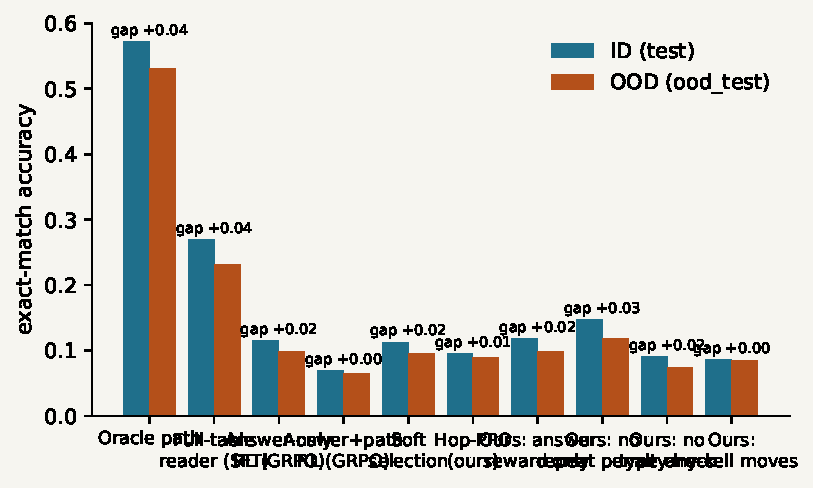
\includegraphics[width=\columnwidth]{../results/figures/F6_id_vs_ood.pdf}
\caption{ID versus OOD EM per method with gap.}
\end{figure}}{}

\section{Reproducibility}
\label{app:repro}

Every run records its seed, configuration, device and code version, per-update training logs and per-question predictions; splits are fixed by question ids and checksums, and an automatic check confirms that no table is shared between splits before evaluation.
All tables and figures are generated from the run logs by scripts, never by hand.
All runs use one pinned software environment.
The full pipeline takes about 12--15 hours on our laptop.

\section{Datasets and Baselines Not Run}
\label{app:cut}

Within the time budget we did not run MultiHiertt \citep{zhao2022multihiertt}, TAT-QA \citep{zhu2021tatqa} or FinQA \citep{chen2021finqa}, a knowledge-graph-style dual-agent baseline inspired by multi-agent path reasoning, a text-generation GRPO baseline with a large language model, potential-based shaping, or more than three seeds.


\end{document}
